\documentclass{article}

\usepackage[utf8]{inputenc}
\usepackage[dvipsnames]{xcolor}
\usepackage{lmodern}
\usepackage{graphicx}
\usepackage{longtable}
\usepackage{tabularx}
\graphicspath{ {../images/} }
\usepackage{imakeidx}
\makeindex[columns=3, title=Alphabetical Index, intoc]

\usepackage{tabularx}
\usepackage{amsmath}
\usepackage{paralist}
\usepackage{enumitem}
\usepackage{hyperref} %\usepackage[hidelinks]{hyperref} %per togliere bordi rossi
\usepackage{makecell}
\usepackage{caption}
\usepackage[maxfloats=256]{morefloats}
\maxdeadcycles=1000

\usepackage[official]{eurosym}
\DeclareUnicodeCharacter{20AC}{\euro{}}

\author{Agosta, Belli, Emili, Giacchini, Luciani}

\begin{document}

\begin{center}
    \sffamily{\fontsize{50}{48} \selectfont \textcolor{red}{Nexi}\textcolor{green}{Fy}}
\end{center}

\begin{center}
    \itshape{\fontsize{20}{48} \selectfont streaming to your pocket}
\end{center}

\bigskip\bigskip\bigskip

\begin{flushleft}
    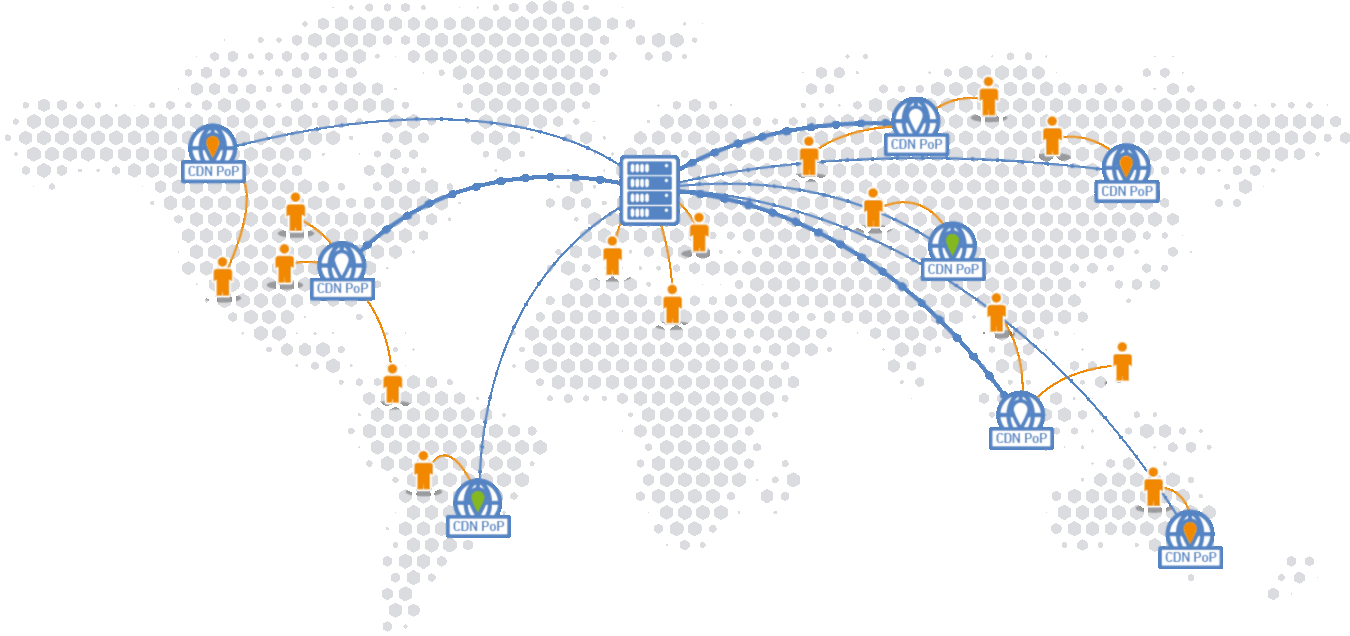
\includegraphics[scale=1]{../images/worldCDN.png}
\end{flushleft}

\bigskip\bigskip\bigskip

\begin{center}
    \itshape{\fontsize{30}{48} \selectfont Stima Dei Costi}
\end{center}

\newpage
\printindex

\newpage
\section{\itshape{Stima dei costi}}
\newcounter{ucCostCounter}
\newcommand{\lastUCCost}{\theucCostCounter}
\newcommand{\nextUCCost}{\stepcounter{ucCostCounter}{\theucCostCounter}}


\newcolumntype{P}[1]{>{\centering\arraybackslash}p{#1}}
\captionsetup[table]{name=Tabella}

Presentiamo una stima dei costi, che utilizza la tecnica dei \emph{Use Case Point (UCP)}, necessaria alla realizzazione del progetto Nexify. Nel seguito effettueremo, nell'ordine:
\begin{itemize}
\item una stima della complessità degli attori;
\item una stima della complessità dei casi d'uso;
\item calcoleremo i fattori di aggiustamento.
\end{itemize}

\noindent \\ Vengono inoltre illustrate le tabelle utilizzate ai fini del calcolo.

\begin{table}[hb]
    \centering
\begin{tabular}{ |P{3.5cm}|P{5cm}|P{3.5cm}|  }
\hline
\textbf{Classificazione dell'attore} & \textbf{Tipo dell'attore} & \textbf{Peso} \\\hline
Semplice & Sistema esterno che interagisce col sistema attraverso un'API	 & 1\\\hline
Medio & Sistema esterno che deve interagire col sistema utilizzando protocolli di comunicazione standard (es. TCP/IP, FTP, HTTP, database) & 2\\\hline
Complesso & Attore umano che accede utilizzando un'interfaccia grafica (GUI)	& 3 \\\hline
\end{tabular}
\caption{Unadjusted Actor Weight (UAW)}
\end{table}

\begin{table}[hb]
    \centering
\begin{tabular}{ |P{3.5cm}|P{5cm}|P{3.5cm}|  }
\hline
\textbf{Tipo di use case} & \textbf{Numero di transazioni} & \textbf{Peso} \\\hline
Semplice & \textless =3 & 5\\\hline
Medio & 4 to 7 & 10\\\hline
Complesso & \textgreater = 8 & 15\\\hline
\end{tabular}
\caption{Unadjusted Use Case Weight (UUCW)}
\end{table}

\begin{table}[hb]
\caption{Attori}
    \centering
\begin{tabular}{ |P{3.5cm}|P{5cm}|P{3.5cm}|  }
\hline
\textbf{ID} & \textbf{Nome} & \textbf{Peso} \\\hline
A\_1.1 & UtenteNonAutenticato & 3\\
A\_1.2 & UtenteAutenticato & 3\\\hline
A\_2.1.1 & ManagerAbbonamenti & 3\\
A\_2.1.2 & ManagerSegnalazioni & 3\\\hline
A\_3 & Pagamento & 1\\\hline
A\_4 & Database & 2\\\hline
A\_5 & CDN & 2\\\hline
A\_6 & Timer & 1\\\hline
\end{tabular}
\caption*{\\\textbf{UAW = 18}}
\end{table}

\clearpage
\begin{longtable}{| p{.20\textwidth} | p{.60\textwidth} | p{.20\textwidth} |} 
\caption{Casi d'uso}\\
\hline
\textbf{ID} & \textbf{Nome} & \textbf{Peso} \\\hline
UC\_\nextUCCost & UC\_CreaAbbonamento & 10\\
UC\_\nextUCCost & UC\_RecuperaAbbonamentiEsistenti & 5\\
UC\_\nextUCCost & UC\_RecuperaServizi & 5\\
UC\_\nextUCCost & UC\_DisattivaAbbonamento & 5\\
UC\_\nextUCCost & UC\_AttivaAbbonamento & 5\\
UC\_\nextUCCost & UC\_AggiungiServizioAbbonamento & 10\\
UC\_\nextUCCost & UC\_RimuoviServizioAbbonamento & 10\\
UC\_\nextUCCost & UC\_RecuperaServiziAbbonamento & 5\\
UC\_\nextUCCost & UC\_RecuperaPianiAbbonamentoUtente & 5\\
UC\_\nextUCCost & UC\_EffettuaPagamentoPartner & 10\\
UC\_\nextUCCost & UC\_CalcolaImportoDaPagare & 5\\
UC\_\nextUCCost & UC\_SospendiAccount & 5\\
UC\_\nextUCCost & UC\_EffettuaRegistrazione & 10\\
UC\_\nextUCCost & UC\_ModificaProfilo & 10\\
UC\_\nextUCCost & UC\_EffettuaLogin &1 0\\
UC\_\nextUCCost & UC\_EffettuaLogout & 5\\
UC\_\nextUCCost & UC\_SottoscriviAbbonamento & 10\\
UC\_\nextUCCost & UC\_DisdiciAbbonamento & 5\\
UC\_\nextUCCost & UC\_CambiaAbbonamento & 15\\
UC\_\nextUCCost & UC\_CreaProdotto & 10\\
UC\_\nextUCCost & UC\_ModificaInformazioniDiBase & 10\\
UC\_\nextUCCost & UC\_CaricaFile & 10\\
UC\_\nextUCCost & UC\_CambiaVisibilit\'aProdotto & 5\\
UC\_\nextUCCost & UC\_RiproduciVideo & 10\\
UC\_\nextUCCost & UC\_RiproduciMusica & 10\\
UC\_\nextUCCost & UC\_PausaPlayer & 5\\
UC\_\nextUCCost & UC\_SpostaPuntoRiproduzionePlayer & 5\\
UC\_\nextUCCost & UC\_SegnalaProdotto & 10\\
UC\_\nextUCCost & UC\_OttieniSegnalazioni & 5\\
UC\_\nextUCCost & UC\_ChiudiSegnalazione & 5\\
UC\_\nextUCCost & UC\_RicercaContenuto & 10\\
UC\_\nextUCCost & UC\_RicercaPopolari & 15\\
UC\_\nextUCCost & UC\_SuggerisciContenuti & 15\\
UC\_\nextUCCost & UC\_VisualizzaPubblicità & 5\\
UC\_\nextUCCost & UC\_CreaPlaylist & 10\\
UC\_\nextUCCost & UC\_AggiungiProdottoPlaylist & 5\\
UC\_\nextUCCost & UC\_RimuoviProdottoPlaylist & 5\\
UC\_\nextUCCost & UC\_CambiaVisibilitáPlaylist & 5\\
UC\_\nextUCCost & UC\_RiproduciPlaylist & 5\\
UC\_\nextUCCost & UC\_AggiungiProdottoAllaCoda & 5\\
UC\_\nextUCCost & UC\_RimuoviProdottoDallaCoda & 5\\
UC\_\nextUCCost & UC\_MostraStatoCoda & 5\\
UC\_\nextUCCost & UC\_RiproduciCoda & 10\\
UC\_\nextUCCost & UC\_CreaSerieTv & 5\\
UC\_\nextUCCost & UC\_CreaAlbum & 5\\
UC\_\nextUCCost & UC\_GestisciScadenzeAbbonamenti & 10\\
UC\_\nextUCCost & UC\_GestisciAbbonamenti & 10\\
UC\_\nextUCCost & UC\_CalcolaQualitáContenuto & 10\\
UC\_\nextUCCost & UC\_OttieniCronologia & 5\\
UC\_\nextUCCost & UC\_DownloadProdotto & 5\\
UC\_\nextUCCost & UC\_RiproduciProdotto & 5\\
UC\_\nextUCCost & UC\_VotaContenuto & 5\\
UC\_\nextUCCost & UC\_CommentaContenuto & 5\\
UC\_\nextUCCost & UC\_RimuoviCommento & 5\\\hline
\caption*{\textbf{UUCW = 400}}
\end{longtable}

\begin{table}[hb]
\caption{Fattori tecnici}
    \centering
        \addtolength{\leftskip} {-2cm}
\begin{tabular}{ |P{2.5cm}|P{5cm}|P{2.5cm}|P{2.5cm}|P{2.5cm}|  }
\hline
\textbf{Fattore} & \textbf{Descrizione} & \textbf{Peso} & \textbf{T factor} & \textbf{Valore} \\\hline
T1 & Sistema distribuito & 2.0 & 4 & 2.0 * 4 = 8.0\\\hline
T2 & Tempo di risposta o obbiettivi di permormance di troughput & 1.0& 4& 1.0 * 4 = 4.0\\\hline
T3 & Efficienza per l'utente finale & 1.0& 3& 1.0 * 3 = 3.0\\\hline
T4 & Complessità del processo interno & 1.0& 3& 1.0 * 3 = 3.0\\\hline
T5 & Il codice deve essere riutilizzabile & 1.0& 2& 1.0 * 2 = 2.0\\\hline
T6 & Facile da installare & 0.5& 4& 0.5 * 4 = 2.0\\\hline
T7 & Facile da usare & 0.5& 5& 0.5 * 5 = 2.5\\\hline
T8 & Portatile & 2.0& 4& 2.0 * 4 = 8.0\\\hline
T9 & Facile da modificare & 1.0& 3& 1.0 * 3 = 3.0\\\hline
T10 & Concorrente & 1.0& 4& 1.0 * 4 = 4.0\\\hline
T11 & Include obbiettivi speciali di sicurezza & 1.0& 2& 1.0 * 2 = 2.0\\\hline
T12 & Fornisce accesso diretto a terze parti & 1.0& 2& 1.0 * 2 = 2.0\\\hline
T13 & Speciali strutture di training sono richieste per l'utente & 1.0& 1& 1.0 * 1 = 1.0\\\hline
\end{tabular}
\caption*{\\\textbf{TFactor = 44.5}}
\end{table}

\begin{table}[hb]
\caption{Fattori ambientali}
    \centering
        \addtolength{\leftskip} {-2cm}
\begin{tabular}{ |P{2.5cm}|P{5cm}|P{2.5cm}|P{2.5cm}|P{2.5cm}|  }
\hline
\textbf{Fattore} & \textbf{Descrizione} & \textbf{Peso} & \textbf{E factor} & \textbf{Valore} \\\hline
F1 & Familiarità con RUP & 1.5 & 1 & 1.5 * 1 = 1.5\\\hline
F2 & Esperienza dell'applicazione & 0.5& 3& 0.5 * 3 = 1.5\\\hline
F3 & Esperienza orientata agli oggetti & 1.0& 3& 1.0 * 3 = 3.0\\\hline
F4 & Capacità di analisi  & 0.5& 4& 0.5 * 4 = 2.0\\\hline
F5 & Motivazione & 1.0& 5& 1.0 * 5 = 5.0\\\hline
F6 & Requisiti stabili & 2.0& 3& 2.0 * 3 = 6.0\\\hline
F7 & Lavoratori part-time & -1.0& 2& -1.0 * 2 = -2\\\hline
F8 & Linguaggio di programmazione difficile & -1.0& 4& -1 * 4 = -4.0\\\hline
\end{tabular}
\caption*{\\\textbf{EFactor = 13.0}\\~\\}
\caption*{\\~\\\large{UUCP = UAW + UUCW = attori + use-case = 18 + 375 = 393}}
\caption*{\\\large{TCF = 0,6 + (0,01 * TFactor) = 0,6 + (0,01 * 44.5) = 1,045}}
\caption*{\\\large{EF = 1,4 + (-0,03 * EFactor) = 1,4 + (-0,03 * 13) = 1,01}}
\caption*{\\\large{UCP = UUCP * TCF * EF = 393 * 1,045 * 1,01 = 414,79185}}
\end{table}

\clearpage

\noindent Considereremo il fattore Hours per UCP \emph{HpUCP} pari a 20, il numero di sviluppatori \emph{dev} che hanno preso parte al progetto pari a 5 e la paga oraria \emph{rate} pari a 50 \$. Da cui:

\vspace{1.0cm}
\centerline{\large{Hours per UCP = HpUCP = 20}}\vspace{0.5cm}
\centerline{\large{Settimane = HpUCP * UCP / (HpW * dev) = 20 * 414,8 / (30 * 5) = 55,3}}\vspace{0.5cm}
\centerline{\large{Paga settimanale = 50 * 30 = 1500 \$}}\vspace{0.5cm}
\centerline{\large{Costo totale = 1500 * 55,3 * 5 = 414.750 \$}}\vspace{0.5cm}
\centerline{\large{Tempo totale ~= 1 anno e 20 giorni}}\vspace{1.0cm}

\noindent Quindi in tutto la realizzazione del nostro progetto richiederà poco più di un anno e verrà a costare circa 414 mila dollari (ovvero circa 370 mila euro).

\begin{table}[b]
\noindent{\large \textbf{Revisioni 9}} \\ \\
\begin{tabular}{|c | c | c | c|} 
 	\hline
	 Numero & Data & Descrizione \\ [0.5ex] 
	\hline\hline
	1 & 20/02/2020 & Stesura iniziale con requisiti funzionali principali \\
	\hline
	2 & 26/02/2020 & Revisione dei principali use case\\
	\hline
\end{tabular}
\end{table}
\index{Index}

\end{document}
